\chapter{Differentialrechnung}
\section{Ableitungen}

def: Die Ableitung \(f'(x)\) einer Funktion gibt die Steigung dieser an einer Stelle \(x\) zurück:
\begin{figure}[H]
    \centering
    \fbox{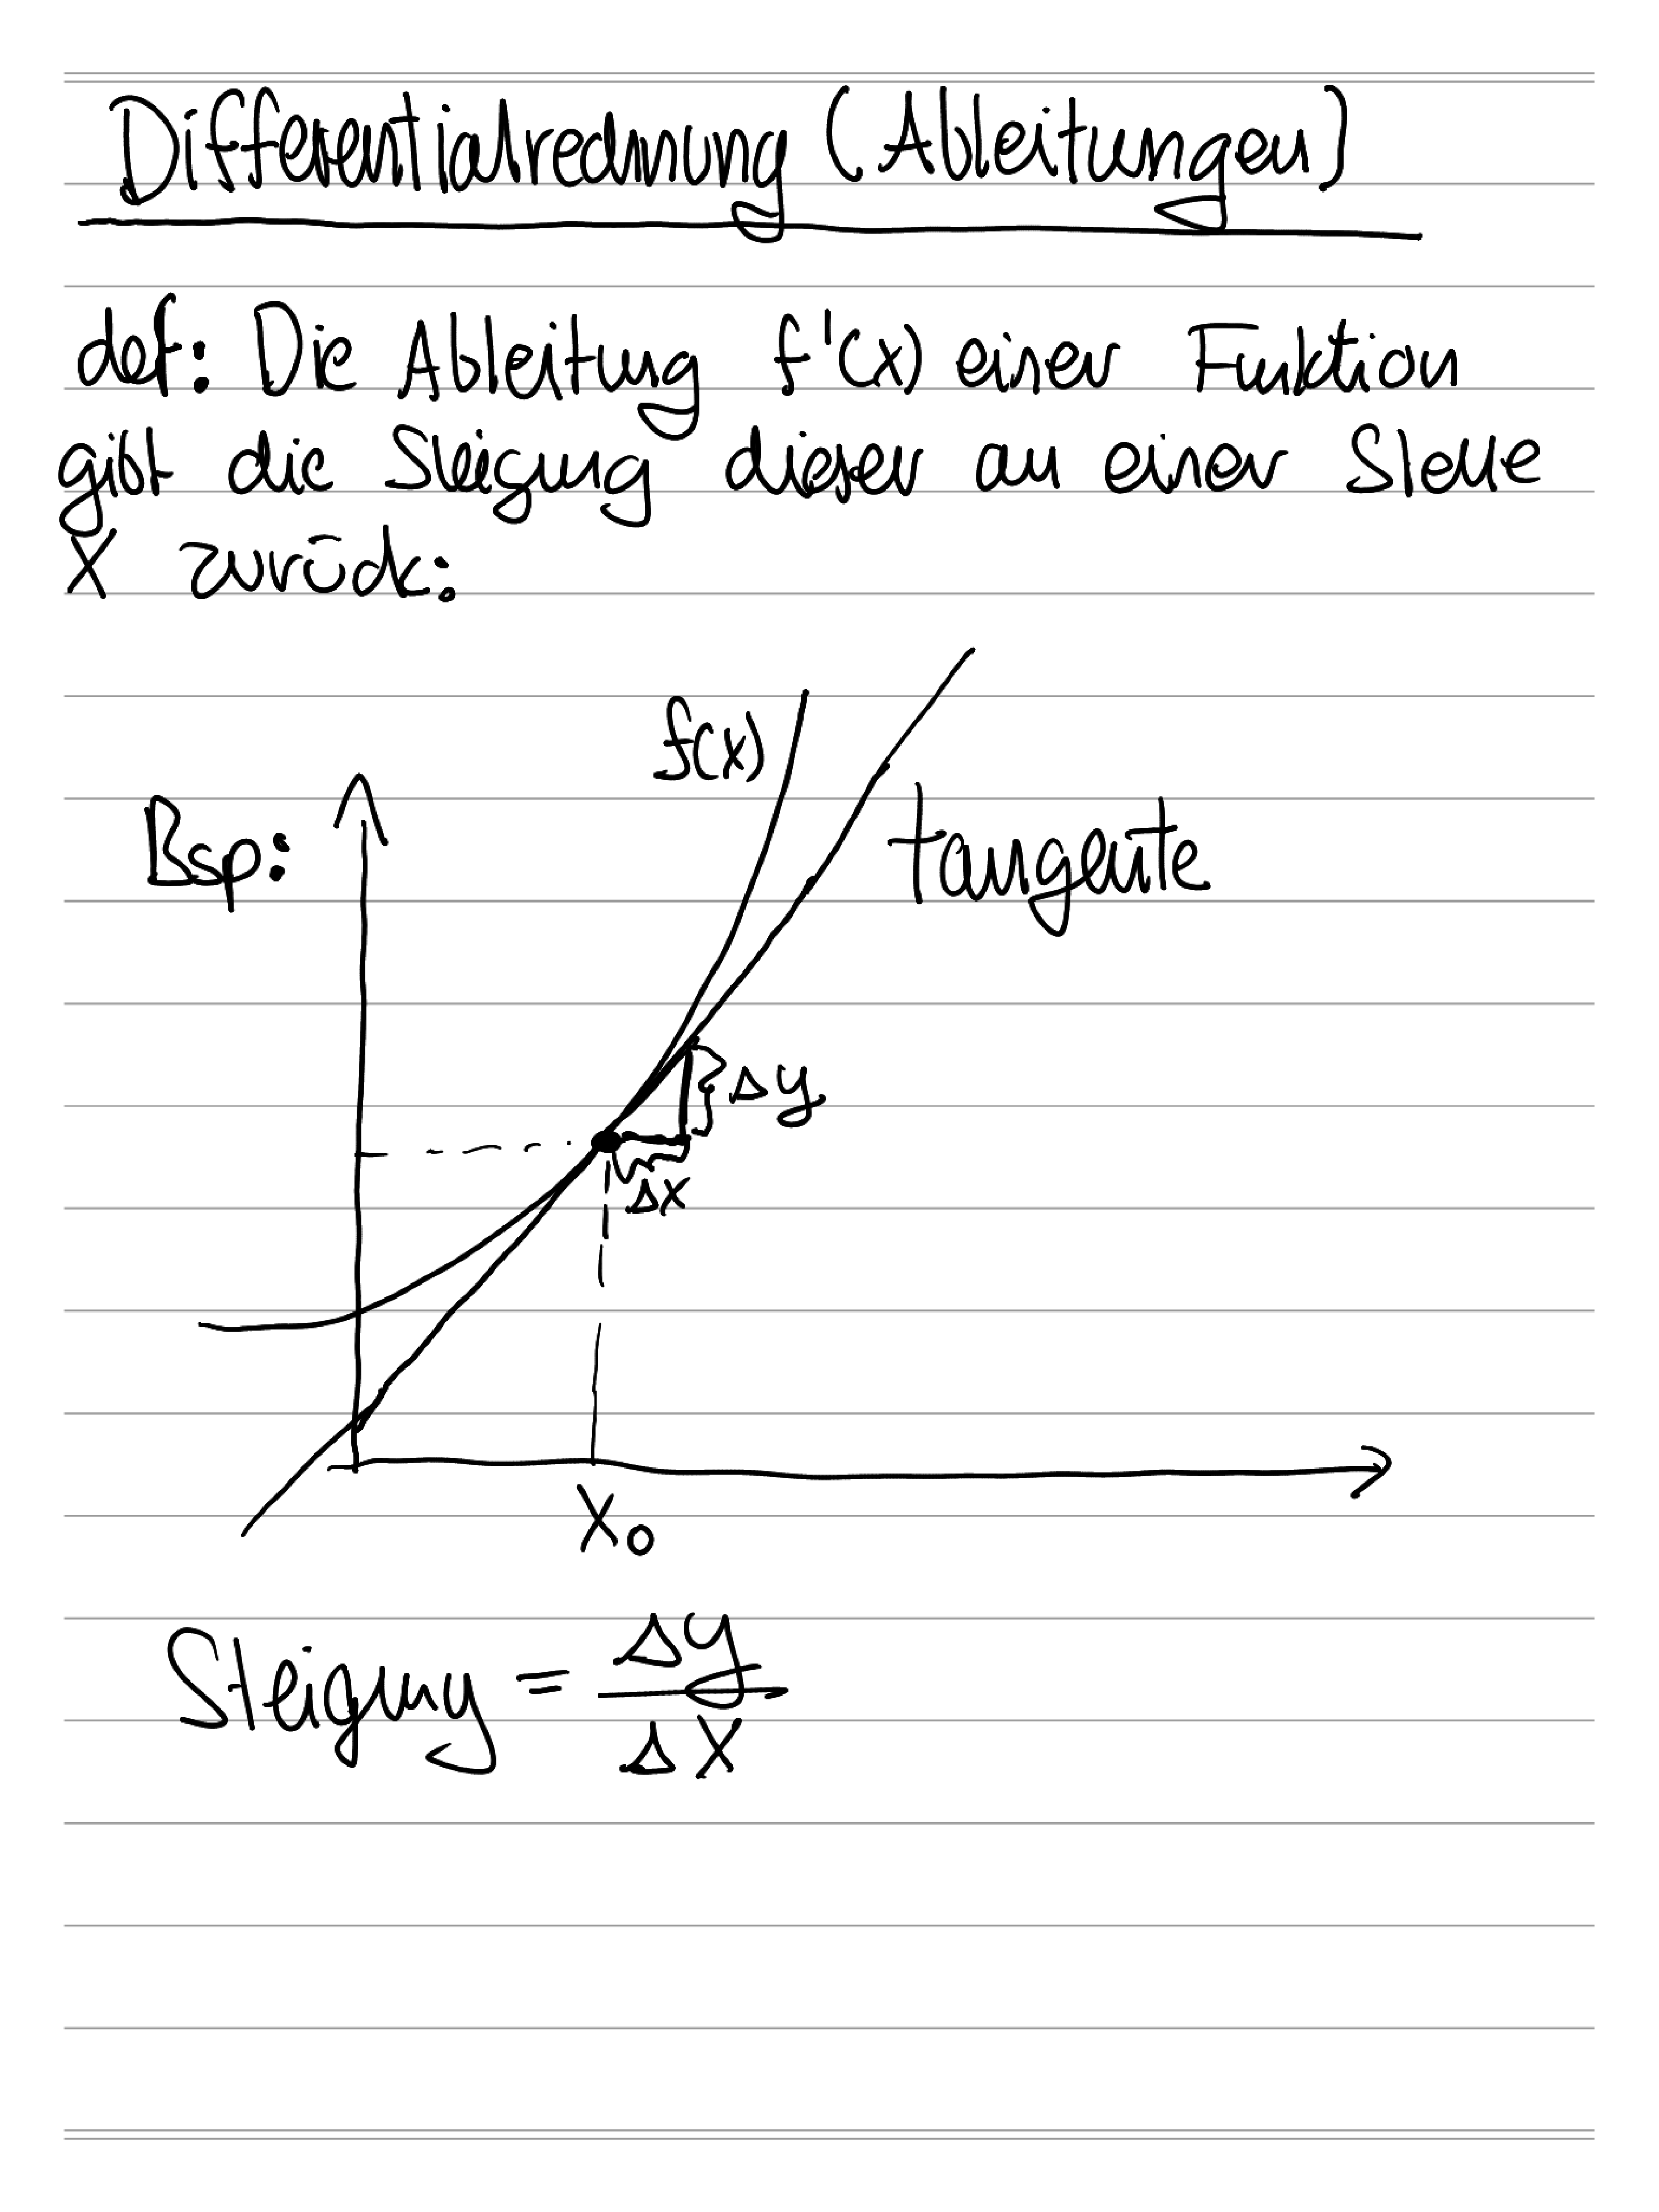
\includegraphics[page=1, height=\textheight, width=.7\linewidth, keepaspectratio, trim=3cm 19cm 6cm 18cm, clip]{./graphics/Ableitungen-1.pdf}}
    \label{figEmpty}
    \caption{Ableitungen-1.pdf Seite 1}
\end{figure}
\begin{equation}
    \text{Steigung} = \frac{\Delta y}{\Delta x}
\end{equation}

Wie können wir die Steigung bestimmen?
\begin{figure}[H]
    \centering
    \fbox{\includegraphics[page=2, height=\textheight, width=.7\linewidth, keepaspectratio, trim=0cm 29.5cm 8cm 7cm, clip]{./graphics/Ableitungen-1.pdf}}
    \label{figEmpty}
    \caption{Ableitungen-1.pdf Seite 2}
\end{figure}
Steigung von \(f(x)\):
\begin{equation}
    f'(x) = \lim_{h\to 0}\frac{f(x+h)-f(x)}{h}
    \eqname{Differentialquotient}
\end{equation}

Beispiel:
\begin{align}
    f(x) &= x^2\\
    \Rightarrow f'(x) &= \lim_{h\to 0}\frac{f(x+h)-f(x)}{h}\\
    &=\lim_{h\to 0}\frac{(x+h)^2-(x)^2}{h}\\
    &=\lim_{h\to 0}\frac{x^2+2xh + h^2 -x^2}{h} \mcomm \text{Binomische Formel}\\
    &=\lim_{h\to 0}\frac{2xh + h^2}{h} \mcomm x^2-x^2=0\\
    &=\lim_{h\to 0}\frac{h \cdot(2x + h)}{h} \mcomm h\text{ ausklammern}\\
    &=\lim_{h\to 0}\frac{\cancel{h} \cdot(2x + h)}{\cancel{h}} \mcomm h\text{ kürzen}\\
    &=\lim_{h\to 0}(2x + h)\\
    &=2x + 0 \mcomm h=0 \text{ einsetzen}\\
    \Rightarrow f'(x) &= 2x
\end{align}
\begin{equation}
    \boxed{f(x) = x^2 \Rightarrow f'(x)=2x}
\end{equation}

Da das sehr aufwendig ist, gibt es einfachere Regeln um Ableitungen zu bestimmen:

Ableitungsregel:
\begin{enumerate}
    \item Potenzregel:
    \begin{align}
        f(x) &= ax^n \quad,\; n \in \R\setminus\{0\}\\ %
        \Rightarrow f'(x) &= n \cdot ax^{n-1} \mcomm \text{"vom Exponenten fällt ein \(n\) vorne dran"}
    \end{align}

    Beispiele:
    % mal sehen ob das auch praktischer geht mit nem anderen environment zb: https://tex.stackexchange.com/a/265686/202560
    \begin{enumerate}
        \item \(x^2 \leadsto 2x\)
        \item \(x^3 \leadsto 3\cdot x^2\)
        \item \(4\cdot x^5 \leadsto 20\cdot x^4\)
        \item \(\sqrt{x} = x^{\nicefrac{1}{2}} \leadsto \frac{1}{2}\cdot x^{-\nicefrac{1}{2}}=\frac{1}{2\sqrt{x}}\)
        \item \(\frac{1}{x^2}=x^{-2} \leadsto -2\cdot x^{-3} = -\frac{2}{x^3}\)
    \end{enumerate}

    \item Summenregel:
    \begin{align}
        f(x) &= g(x) + h(x)\\
        \Rightarrow f'(x) &= g'(x) + h'(x) \mcomm \text{Summanden einzeln ableiten!}
    \end{align}
    Beispiele:
    \begin{enumerate}
        \item \(x^2 + 3x^3 \leadsto 2x + 9x^2\)
        \item \(x + x^2 + 4x^4 \leadsto 1 + 2x + 16x^3\)
    \end{enumerate}
    \item Produktregel:
    \begin{align}
        f(x) &= g(x) \cdot h(x)\\
        \Rightarrow f'(x) &= g'(x) \cdot h(x) + g(x) \cdot h'(x)
    \end{align}
    Beispiele:
    \begin{enumerate}
        \item \(x \cdot x \leadsto 1 \cdot x + x \cdot 1 = 2x \)
        \item \(x \cdot \sin(x) \leadsto 1 \cdot \sin(x) + x \cdot \cos(x)\)
        \item \(3x^4 \cdot \e^x \leadsto 12x^2\e^x + 3x^4\e^x\)
    \end{enumerate}
    \item Kettenregel:
    \begin{figure}[H]
        \centering
        \fbox{\includegraphics[page=6, height=\textheight, width=.7\linewidth, keepaspectratio, trim=0cm 0cm 0cm 0cm, clip]{./graphics/Ableitungen-1.pdf}}
        \label{figEmpty}
        \caption{Ableitungen-1.pdf Seite 6}
    \end{figure}
\end{enumerate}


\begin{figure}[H]
    \centering
    \fbox{\includegraphics[page=7, height=\textheight, width=.7\linewidth, keepaspectratio, trim=0cm 0cm 0cm 0cm, clip]{./graphics/Ableitungen-1.pdf}}
    \label{figEmpty}
    \caption{Ableitungen-1.pdf Seite 7}
\end{figure}

\begin{figure}[H]
    \centering
    \fbox{\includegraphics[page=8, height=\textheight, width=.7\linewidth, keepaspectratio, trim=0cm 0cm 0cm 0cm, clip]{./graphics/Ableitungen-1.pdf}}
    \label{figEmpty}
    \caption{Ableitungen-1.pdf Seite 8}
\end{figure}
